% !TEX encoding = UTF-8 Unicode
\documentclass[a4paper]{article}

\usepackage{color}
\usepackage{xcolor}
\usepackage{url}
\usepackage[T2A]{fontenc} % enable Cyrillic fonts
\usepackage[utf8]{inputenc} % make weird characters work
\usepackage{graphicx}
\usepackage{listings}
\usepackage[english,serbian]{babel}
\usepackage{booktabs}
\usepackage{multicol}
%\usepackage[english,serbianc]{babel} %ukljuciti babel sa ovim opcijama, umesto gornjim, ukoliko se koristi cirilica

\usepackage[unicode]{hyperref}
\hypersetup{colorlinks,citecolor=green,filecolor=green,linkcolor=blue,urlcolor=blue}

%\newtheorem{primer}{Пример}[section] %ćirilični primer
\newtheorem{primer}{Primer}[section]

\definecolor{mygreen}{rgb}{0,0.6,0}
\definecolor{mygray}{rgb}{0.5,0.5,0.5}
\definecolor{mymauve}{rgb}{0.58,0,0.82}
\definecolor{commentgreen}{RGB}{2,112,10}
\definecolor{eminence}{RGB}{108,48,130}
\definecolor{weborange}{RGB}{255,165,0}
\definecolor{frenchplum}{RGB}{129,20,83}
\definecolor{pink}{rgb}{0.858,0.188,0.478}

\lstdefinelanguage{Elixir}{
    morekeywords={case,catch,def,do,else,false,%
        use,alias,receive,timeout,defmacro,defp,%
        for,if,import,defmodule,defprotocol,%
        nil,defmacrop,defoverridable,defimpl,%
        super,fn,raise,true,try,end,with,%
        unless},
    otherkeywords={<-,->, |>, \%\{, \}, \{, \, (, )},
    keywords=[2]{IO},
    keywords=[3]{iex},
    sensitive=true,
    morecomment=[l]{\#},
    morecomment=[n]{/*}{*/},
    morecomment=[s][\color{purple}]{:}{\ },
    morestring=[s][\color{orange}]"",
    commentstyle=\color{commentgreen},
    keywordstyle=\color{eminence},
    keywordstyle=[2]\color{pink},
    keywordstyle=[3]\color{mygreen},
    stringstyle=\color{red},
	basicstyle=\ttfamily,
	breaklines,
	showstringspaces=false,
	frame=none
}

\lstset{ 
  backgroundcolor=\color{white},   % choose the background color; you must add \usepackage{color} or \usepackage{xcolor}; should come as last argument
  basicstyle=\scriptsize\ttfamily,        % the size of the fonts that are used for the code
  breakatwhitespace=false,         % sets if automatic breaks should only happen at whitespace
  breaklines=true,                 % sets automatic line breaking
  captionpos=b,                    % sets the caption-position to bottom
  commentstyle=\color{mygreen},    % comment style
  deletekeywords={...},            % if you want to delete keywords from the given language
  escapeinside={\%*}{*)},          % if you want to add LaTeX within your code
  extendedchars=true,              % lets you use non-ASCII characters; for 8-bits encodings only, does not work with UTF-8
  %firstnumber=1,                % start line enumeration with line 1000
  frame=none,	                   % adds a frame around the code
  keepspaces=true,                 % keeps spaces in text, useful for keeping indentation of code (possibly needs columns=flexible)
  keywordstyle=\color{blue},       % keyword style
  language=Elixir,                 % the language of the code
  morekeywords={*,...},            % if you want to add more keywords to the set
  numbers=none,                    % where to put the line-numbers; possible values are (none, left, right)
  numbersep=5pt,                   % how far the line-numbers are from the code
  numberstyle=\tiny\color{mygray}, % the style that is used for the line-numbers
  rulecolor=\color{black},         % if not set, the frame-color may be changed on line-breaks within not-black text (e.g. comments (green here))
  showspaces=false,                % show spaces everywhere adding particular underscores; it overrides 'showstringspaces'
  showstringspaces=false,          % underline spaces within strings only
  showtabs=false,                  % show tabs within strings adding particular underscores
  stepnumber=1,                    % the step between two line-numbers. If it's 1, each line will be numbered
  stringstyle=\color{mymauve},     % string literal style
  tabsize=2,	                   % sets default tabsize to 2 spaces
  %title=\lstname                   % show the filename of files included with \lstinputlisting; also try caption instead of title
}

\begin{document}

\title{Programski jezik Elixir\\ \small{Seminarski rad u okviru kursa\\Metodologija stručnog i naučnog rada\\ Matematički fakultet}}

\author{Božidar Antić, Marija Novaković,\\ Srđan Lazarević, Radmila Ninković\\bozidar\_antic@matf.bg.ac.rs, mi14170@alas.matf.bg.ac.rs,\\ mi14126@alas.matf.bg.ac.rs, mi14202@alas.matf.bg.ac.rs}

%\date{9.~april 2015.}

\maketitle

\abstract{
U ovom radu je obrađen funkcionalni programski jezik Elixir. Ukratko je predstavljena istorija jezika, Erlang virtualna mašina i osnove jezika. Objašnjeni su ugrađeni tipovi, anonimne i imenovane funkcije, konkurentnost i moduli. Opisana je instalacija i navedeni su primeri za lakše upoznavanje sa jezikom, kao i poznata okruženja koja se koriste u radu sa Elixir programskim jezikom.  
}

\tableofcontents

\newpage

\section{Uvod}
\label{sec:uvod}

Elixir je dinamičan, funkcionalni programski jezik koji se pokreće na Erlang vituelnoj mašini pa samim tim i deli pogodna svojstva kao što su konkurentnost i tolerisanje grešaka, koje dolaze sa ovim okruženjem.\cite{knjigaElixir} Iz tačke gledišta olakšavanja svakodnevnog razvoja sofvera, koncepti kao što su metaprogramiranje - tehnika kojom programi imaju mogućnost da druge programe posmatraju kao svoje podatke i na taj način čitaju pa čak i modifikuju njihov, a samim tim i svoj kôd u vreme izvršavanja, zatim polimorfizam i makroi kao i podrška za alate, su falili Erlangovom ekosistemu, i upravo je Elixir to nadomestio. Cilj ovog rada je da čitaoca bliže upozna sa osnovnim osobinama, funkcionalnostima i specifičnostima ovog jezika kao i da kroz primere pokuša da približi programerske prakse korišćene u ovom jeziku.

\section{Istorijat}
\label{sec:istorijat}

Tokom 2010. godine, José Valim, u to vreme zaposlen na poziciji programera u kompaniji Plataformatec, radio je na poboljšanju performansi Ruby on Rails framework-a na višejezgarnim sistemima. \cite{sitePlataformatec} Shvatio je da Ruby nije bio dovoljno dobro dizajniran da reši problem konkurentnosti, pa je započeo istraživanje drugih tehnologija koje bi bile prihvatljivije. Tako je otkrio Erlang, i upravo ga je interesovanje prema Erlangovoj virtuelnoj mašini podstaklo da započne pisanje Elixira. Uticaj projekta na kome je do tada radio odrazio se na to da Elixir ima sintaksu koja je nalik na Ruby-jevu. Ovaj jezik se pokazao veoma dobro pri upravljanju milionima simultanih konekcija: u 2015. je zabeleženo upravljanje nad 2 miliona WebSocket konekcija \cite{sitePhoenix}, dok je u 2017. za skalirani Elixir zabeležena obrada 5 miliona istovremenih korisnika. Elixir se danas koristi u velikim kompanijama, kao što su Discord \cite{siteDiscord} i Pinterest\cite{sitePinterest}.

\section{BEAM - Erlang virtualna mašina}

Originalno BEAM je bila skraćenica za Bogdan's Erlang Abstract Machine, po Bogumil "Bogdan" Hausman koji je napisao originalnu verziju virtualne mašine, ali ime se takođe može tumačiti kao Björn's Erlang Abstract Machine, po Björn Gustavsson, koji piše i održava trenutnu verziju.

Kako je Elixir zapravo nastao proširivanjem funkcionalnosti BEAM-a (Erlangove virtualne mašine), sa ciljem da se zadrži kompatibilnost sa Erlang ekosistemom, važno je opisati osnovne koncepte funkcionisanja Erlang virtualne mašine na kojoj se kompajlirani Elixir kôd izvršava.

BEAM predstavlja jezgro Erlang Open Telecom Platform (Erlang/OTP), platforme koja se sastoji od Erlang Run-Time System(ERTS) i  kolekcije unapred kompajliranih biblioteka i alata pisanih u Erlangu, sto omogućava Elixiru direktno korišćenje funkcionalnosti koje pružaju Erlang moduli.

ERTS predstavlja modul zadužen za kompilaciju Erlang i Elixir izvornog kôda u bytecode koji se onda izvršava u okviru BEAM-a.

U okviru BEAM-a, sav kôd se izvršava u sitnim konkurentnim procesima, pri čemu procesi nisu procesi operativnog sistema, vec Erlang procesi, što je moguće upravo zbog izvršavanja u okviru BEAM virtualne mašine. Svaki od procesa je memorijski nezavistan i sva međuprocesna komunikacije se odvija razmenjivanjem poruka, čime se obezbeđuje koncept konkurentnosti slanjem poruka \textit{(eng. message passing concurrency)}.\cite{knjigaElixir} 

Prevođenjem Elixir izvornog fajla generiše se .beam fajl koji sadrži bytecode koji se može izvršavati u okviru BEAM-a.

\section{Osobine jezika} 
\label{sec:osobine}
U ovom poglavlju će biti opisane osobine Elixira, osnove njegove sintakse, semantike, kao i podrška za osnovne koncepte funkcionalnih jezika poput poklapanja obrazaca (eng.~{\em Pattern matching}) i imutabilnosti podataka. \cite{knjigaElixir}\cite{knjigaElixir2}

Pre nego što započnemo priču o tipovima, treba pomenuti \textbf{Kernel}. To je podrazumevano okruženje koje se koristi u Elixiru. Ono sadrži primitive jezika kao što su: \textit{aritmetičke operacije}, rukovanje \textit{procesima} i \textit{tipovima}, \textit{makroe} za definisanje novih funkcionalnosti (\textit{funkcija, modula...}), provere \textit{guard-ova} - predefinisanog skupa funkcija i makroa koji proširuju mogućnost \textit{pattern matching}-a itd.\cite{siteElixir} 

\subsection{Poklapanje obrazaca}
\label{sec:pattern}
Poklapanje obrazaca je proveravanje da li se u data sekvenci tokena može prepoznati neki šablon. Na praktičnom primeru operatora = ovaj koncept će biti jasniji. 
U većini programskih jezika, operator = je operator dodele, koji levoj strani dodeljuje vrednost izraza na desnoj. U Elixiru se naziva operator \textit{uparivanja} (eng.~{\em matching}). On se uspešno izvršava ako pronađe način da izjednači levu stanu (svoj prvi operand) sa desnom (drugi operand).
\begin{primer}
U narednom parčetu kôda \textit{a} je promenljiva, koju Elixir uspeva da izjednači sa vrednoću 1, tako što biva postavljena na tu vrednost. U drugoj naredbi izvršavanje operacije ponovo uspeva jer je vrednost leve strane 1 dok promenljiva sa desne strane već ima vrednost 1 zbog prethodne operacije. Sledeća naredba ne uspeva jer Elixir pokušava da izjednači levu stranu, koja je broj 2, koji može imati samo tu vrednosti, sa promenjivom \textit{a} koja ima vrednost 1. Ključna stvar za razumeti je da Elixir ne pokušava da izjednači levu \textit{i} desnu stranu, već levu \textit{sa} desnom.
\end{primer}
\begin{lstlisting}[caption={Primer jednostavnog poklapanja obrazaca},frame=none, label=simple]
iex> a = 1
#out: 1
iex> 1 = a
#out: 2
iex> 2 = a
#out:(MatchError) no match of right hand side value: 1
\end{lstlisting}

\subsection{Imutabilnost}
\label{sec:tipovi}
Imajući na umu funkcionalnu paradigmu Elixira, imutabilnost podataka je osobina koja je neizostavna. Naime, jednom kreirani podaci ne mogu biti promenjeni. Bez ulaženja u dublje analize rasprava o tome da li je mutabilnost podataka dobra ili loša, činjenica je da postojanje stanja, i funkcija koje to stanje mogu menjati u izrazima sa bočnim efektima, otežava razumevanje i još bitnije, utvrđivanje korektnosti funkcionisanja sistema. Pogotovo u slučaju višenitnih, konkurentnih ili distribuiranih programa, kakvi se najčešće pišu korišćenjem Elixir programskog jezika. %\cite{knjigaElixir} \cite{knjigaElixir2}

\subsection{Ugrađeni tipovi}
\label{sec:tipovi}
Elixir implementira desetine tipova. Od njih je važno istaći ugrađene - primitivne tipove, preko kojih su realizovane implementacije ostalih:
\begin{multicols}{2}
\begin{itemize}
  \item Atomi (\textit{Atom})
  \item Celi brojevi (\textit{Integer})
  \item Brojevi u pokretnom zarezu (\textit{Float})
  \item Procesi (\textit{Process})
  \item Portovi (\textit{Port})
  \item Uređene torke (\textit{Tuple})
  \item Liste (\textit{List})
  \item Mape (\textit{Map})
  \item Funkcije (\textit{Function})
  \item Niske bitova 
  \item Reference
\end{itemize}
\end{multicols}

U zagradama nakon tipa, osim u poslednja dva koji nemaju odgovarajuće module, navedena su imena modula koji sadrže funkcije koje se koriste za operacije nad tim tipom. Imena ovih modula ne treba mešati sa primitivnim tipovima navedenim gore, iako oni sami predstavljaju tip. Oni se mogu zamisliti kao neka vrsta omotača oko primitivnog tipa koji obezbeđuje bogatije funkcionalnosti nad njime. 
\begin{primer}
Literal [...] može biti iskorišćen da se napravi lista (primitiva), nad njom je moguće iskoristiti operator | koji bi je dekomponovao na glavu i rep ili od nje napravio novu listu. U modulu \textit{List} imamo funkciju \textit{last} koja kada se primeni na listu, kao rezultat vraća njen poslednji element.
\end{primer}

Može biti čudno što se na ovoj listi nisu našle niske ili strukture, ali one su deo složenih tipova podržanih od strane Elixira. Takođe, postoji debata o tome da li su regularni izrazi i opsezi (\textit{Ranges}) tipovi za sebe i u nekoj literaturi se posmatraju ovako iako su tehnički strukture. \cite{knjigaElixir}

\subsubsection{Atomi, celi i brojevi u pokretnom zarezu i opsezi}
\label{sec:ime}
\textit{Atomi} su konstante koje predstavljaju ime. Počinju dvotačkom i njihovo ime im je i vrednost, što znači da će dva atoma sa istim imenom pri poređenju uvek biti isti bez obzira na to da li su kreirani od strane različitih aplikacija ili procesa.

\textit{Celi brojevi} su slični kao i u većini drugih jezika i mogu se obeležavati korišćenjem dekadne (1234), heksadekadne (0xcafe), oktalne (0o1234) i binarne (0b1010) notacije. Karakter \_ se može koristiti za odvajanje blokova cifara. Bitna stvar je da ne postoji fiksna veličina za čuvanje celih brojeva u memoriji, već interna reprezentacija raste kako bi obezbedila da broj bude smešten u celosti.

\textit{Brojevi u pokretnom zarezu} se u memoriji zapisuju po standardu IEEE 754 \cite{knjigaElixir}\cite{siteIEEE}, a za zapisivanje konstanti ovog tipa koristi se tačka između najmanje dve cifre. Takođe je moguće koristiti i notaciju koja obuhvata navođenje eksponenta.

\subsubsection{Procesi, portovi, reference i niske bitova}
\label{sec:ime}
\textit{Procesi} predstavljaju pogodnost za rad sa nitima.

\textit{Portovi} su reference na spoljne resurse koji omogućavaju interakciju sa spoljnim svetom.

\textit{Reference} su jedinstvene vrednosti u globalnom kontekstu izvršavanja programa koje se kreiraju pozivom make\_ref funkcije.

\subsubsection{Torke}
\label{sec:ime}
\textit{Torke} su zamišljene kao kontejneri elemenata fiksne dužine koji bi trebalo da sadrže svega nekoliko elemenata. Osnovna stvar koja ih razlikuje od \textit{listi} je u semantici njihove upotrebe. \textit{Liste} se koriste kada se manipuliše kolekcijom, dok se operacija čitanja elementa iz \textit{torke} izvršava u konstantnom vremenu, pa se uglavnom koristi kako bi se u nju smestile povratne vrednosti funkcije. Može da sadrži elemente različitog tipa i ove vrednosti su u memoriji zapisane jedna za drugom.%\cite{knjigaElixir}\cite{knjigaElixir2}

\subsubsection{Liste}
\label{sec:ime}
\textit{Lista} je kolekcijski tip koji je imlementiran kao povezana lista. Ova osobina čini da je pristup proizvoljnom elementu složenosti \( O(n) \). Lista može biti prazna ili sastavljena od glave i tela, gde je glava element liste, a telo je lista. Primećuje se rekurzivna definicija liste koja je zajedno sa operacijom izdvajanja glave od tela (koja je pritom efikasna znajući strukturu implementacije) osnov za mnoge programerske prakse u Elixiru. Pošto je kao i svi podaci, lista u Elixiru imutabilna, čitalac može pomisliti da će pri prethodno navedenoj operaciji biti napravljena nova lista koja će predstavljati rep prethodne. Ovo bi bilo memorijski, pa i vremenski vrlo neefikasno pa je u elixiru implementirano tako što će umesto nove liste biti vraćen pokazivač na rep prethodne.%\cite{knjigaElixir}\cite{knjigaElixir2}

\subsubsection{Mape}
\label{sec:ime}
\textit{Mapa} je kolekcija koja sadrži parove ključeva i vrednosti. Glavna razlika između liste parova ključeva i vrednosti, i mape leži u tome da je mapa asocijativna struktura podataka i samim tim ne dozvoljava duplirane vrednosti ključa. Mapa je vrlo efikasna, pogotovo sa rastom količine podataka. Ukoliko je potrebno da u kolekciji podaci ostanu u redosledu u kome su navedeni pri inicijalizaciji, lista parova je bolji izbor. One se najčešće koriste kako bi se funkcijama prosledile opcije. U ostalim slučajevima, mapa je uglavnom bolji izbor.%\cite{knjigaElixir}\cite{knjigaElixir2}
\begin{primer}
Primer inicijalizacije liste parova ključeva i vrednosti, i mape sa istim vrednostima. Za listu je korišćena skraćenica obezbeđena u Elixiru zbog čestog koriščenja ovog kontrukta. Parovi u listi su tipa torke, ključevi su atomi dok su vrednosti niske.
\end{primer}
\begin{lstlisting}[caption={Primer liste parova ključeva i vrednosti, i mape},frame=none, label=simple]
list = [key1: "value1", key2: "value2", key3: "value3"]
# interno: [ {:key1,"value1"}, {:key2,"value2"}, {:key3,"value3"} ]
map = %{:key1 => "value1",:key2 => "value2",:key3 => "value3"}
\end{lstlisting}

\subsection{Anonimne funkcije}
Anonimne funkcije su u Elixiru kao i u drugim funkcionalnim programskim jezicima građani prvog reda. Iako explicitno nisu imenovane, na funkcije ove vrste se možemo referisati tako što ih sačuvamo u promenljivoj. Takođe, zanimljivo je da anonimne funkcije mogu imati više tela, odnosno različite implementacije u zavisnosti od broja ili vrednosti parametara. Ova funkcionalnost, koja poznavaoce objektno orijentisanog programiranja može podsetiti na koncept preopterećivanja (eng.~{\em overloading}) metoda, je ostvarena pomoću poklapanja obrazaca.
\begin{primer}
Naredna anonimna funkcija pokušava da ispiše prvu liniju fajla čije je ime prosleđeno kao argument, a ukoliko fajl ne postoji ispisuje poruku o grešci.
\end{primer}
\begin{lstlisting}[caption={Primer anonimne funkcije}, label=simple]
handle_open = fn
    {:ok, file} -> "Read data: #{IO.read(file, :line)}"
    {_, error}  -> "Error: #{:file.format_error(error))}"
end
\end{lstlisting}
\label{sec:ime}

\subsection{Moduli i imenovane funkcije}
\label{sec:ime}
Kada program sadrži previše linija kôda, poželjno je strukturirati ga. U Elixir-u kôd se može izdvojiti u imenovane funkcije koje se dalje organizuju u module, čak šta više moraju se pisati u okviru njih. 
Jednostavan primer modula Times koji sadrži jednu funkciju, double, prikazan je ispod. 
%\begin{verbatim}
\begin{lstlisting}[caption={Množenje broja sa 2}, label=simple]
defmodule Times do
    def double(n) do
        n * 2
    end
end   
\end{lstlisting}

Jedan način grupisanja izraza i prosleđivanje istih drugom kôdu je do..end blok. Koristi se u modulima, imenovanim funkcijama, strukturama kontrole (eng.~{\em control structures}) i na bilo kom drugom mestu gde kôd treba da se koristi kao entitet. Može se proslediti i više linija grupisanjem zagradama:
\begin{lstlisting}[caption={Ispisivanje poruke pozdrava}, label=simple]
def greet(greeting, name), do: (
    IO.puts greeting
    IO.puts "How're you doing, #{name}?"
)
\end{lstlisting}

\subsubsection{Pozivi funkcija i poklapanje obrazaca}
Za razliku od anonimnih funkcija u ovom slučaju moramo pisati funkciju više puta, svaki put sa listom parametara i telom funkcije. Kada se funkcija pozove, Elixir pokušava da poklopi argumente sa listom parametara prve definicije, ukoliko ne može da ih poklopi nastavlja sa sledećom definicijom iste funkcije itd. dok ne nađe pravog kandidata.
Važno je obratiti pažnju na redosled pisanja funkcija jer Elixir uvek pokušava od vrha ka dole i izvršava se prva koja se poklopila.

\subsubsection{Čuvari (eng.~{\em Guards})}
Poklapanje obrazaca omogućava Elixir-u da odluči koju funkciju će pozvati na osnovu argumenata koji su prosleđeni. Međutim ukoliko treba razlikovati na osnovu tipova ili na osnovu nekih testova koji uključuju vrednosti koristimo čuvare. To su zapravo predikati koji su pridruženi definiciji funkcije koristeći ključnu reč when jednom ili više puta. 

\subsubsection{Podrazumevani parametri}
Kada se definiše imenovana funkcija  može se dati podrazumevana vrednost bilo kom parametru korišćenjem sintakse  param \textbackslash \textbackslash  vrednost. Pri pozivu funkcije koja ima podrazumevane vrednosti, poredi se broj argumenata koji se prosleđuju sa brojem obaveznih vrednosti. Ukoliko je broj argumenata manji  nema poklapanja. Ukoliko je njihov broj jednak, obavezne vrednosti uzimaju vrednosti argumenata, a ostali parametri uzimaju podrazumevane vrednosti. U slučaju da je broj prosleđenih argumenata veći od obaveznih, Elixir može da pregazi podrazumevane vrednosti nekih ili svih parametara tako što ide sa leva na desno.
\begin{lstlisting}[caption={Poziv funkcije sa podrazumevanim parametrima}, label=simple]
defmodule Example do
    def func(p1, p2 \\ 2, p3 \\ 3, p4) do
        IO.inspect [p1, p2, p3, p4]
    end
end
Example.func("a", "b") # => ["a",2,3,"b"]
Example.func("a", "b", "c") # => ["a","b",3,"c"]
Example.func("a", "b", "c", "d") # => ["a","b","c","d"]
\end{lstlisting}

\subsubsection{Operator prosleđivanja |> (eng.~{\em pipe})}
Operator |> uzima rezultat izraza sa leve strane i ubacuje ga kao prvi parametar poziva funkcije sa desne strane. U suštini val |> f(a, b) je isto što i f(val, a, b).

\subsubsection{Direktive u okviru modula}
\begin{itemize}
    \item Import direktiva - dovlači funkcije i makroe nekog modula u trenutni opseg; eliminiše se potreba za ponavljanjem imena modula. Only: ili except: su opcioni parametri  praćeni  listom parova naziv:broj parametara. Pogodni su za kontrolu koje funkcije ili makroi su importovani.
    \begin{lstlisting}[nolol=true]
    import Module [, only: | except: ]
    \end{lstlisting}
    \item Alias direktiva - kreira alias za modul i samim tim skraćuje pisanje.
    Na primer:
    \begin{lstlisting}[nolol=true]
    alias My.Other.Module.Parser, as: Parser
    \end{lstlisting}
    \item Require direktiva - obezbeđuje da su definicije makroa dostupne prilikom prevođenja.
\end{itemize}

\subsubsection{Atributi modula}
Atributom modula se naziva svaka stavka metapodatka i identifikovan je imenom. U okviru modula može se pristupiti atributu stavljajući prefiks ‘@’  ispred imena. Dodeljivanje vrednosti atributu vrši se sa @ime vrednost i ono se ne može obavljati u okviru funkcije. Ovi atributi nisu promenljive u konvencionalnom smislu, i uglavnom se upotrebljavaju kao što Java ili Ruby programeri upotrebljavaju konstante.

\subsection{Konkurentnost}
Jedna od glavnih karakteristika Elixir-a je ideja o pakovanju kôda u male celine koje se mogu pokretati nezavisno i istovremeno. Elixir za konkurentnost koristi model {\em actor}. {\em Actor} je nezavistan proces koji ništa ne deli sa bilo kojim drugim. Mogu se napraviti novi, poslati im poruke i primiti poruku nazad. Procesi se mogu izvoditi na svim jezgrima procesora, imaju malo dodatnih troškova. Lako je napraviti i nekoliko stotina hiljada procesa čak i na slabijim računarima. 

Procesi podrazumevano nisu povezani, pa samim tim nisu svesni stanja kroz koje prolaze drugi procesi. Pomoću funkcije spawn\_link pravi se novi proces koji je povezan sa roditeljskim i kroz mehanizme povezivanja (eng.~{\em linking}) i nadgledanja (eng.~{\em monitoring}) mogu komunicirati.

Ukoliko želimo da obezbedimo distribuirano izvršavanje naših programa, Elixir obezbeđuje koncept čvorova izvršavanja. Čvorovi nisu svesni postojanja drugih dok se eksplicitno ne povežu. Ukoliko su čvorovi povezani, izvršavanje i npr. obrada rezultata jednog procesa se mogu odvijati na različitim, potencijalno kilometrima udaljenim računarima. \cite{knjigaElixir}

Na slici \ref{fig:procesi} prikazana je zavisnost vremena potrebnog da se procesi naprave u odnosu na njihov broj. Grafik je iscrtan na logaritamskoj skali pa na prvi pogled možda nije očigledno da rast prati linearni trend. Informacije o programu koji je pokretan kao i mašini na kojoj je izvršavan nalaze se u Dodatku \ref{sec:apendix}. 

\begin{figure}[h!]
\begin{center}
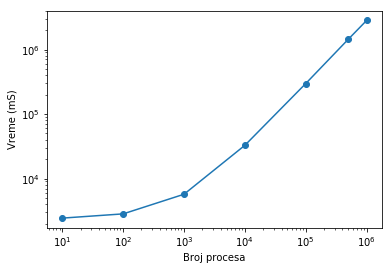
\includegraphics[scale=0.75]{plot.png}
\end{center}
\caption{Grafik potrebnog vremena za pravljenje procesa}
\label{fig:procesi}
\end{figure}

\section{Instalacija}
Pre instalacije Elixira neophodno je instalirati Erlang na odgovarajućem operativnom sistemu. Mnogi različiti upravljači paketima (apt, dnf, pkg, pacman, MacPorts, Homebrew, itd.) uključuju Erlang. On je sve više deo standardne instalacije na mnogim sistemima, uključujući i Ubuntu, uglavnom zahvaljujući širenju CouchDB-a. Nakon instalacije Erlang-a može se instalirati Elixir. 

\subsection{Linux}    
Ako koristite operativni sistem Linux, Elixir se može instalirati komandom {\em sudo apt-get install elixir}\cite{siteElixir}. Nakon instalacije, Elixir programi se mogu kompajlirati i pokretati u interpreteru. Kôd iz datoteke se može kompajlirati komandom {\em elixir} iza koje se navodi ime fajla sa ekstenzijom {\em .exs}.

\subsection{Windows}    
Ako koristite operativni sistem Windows, instaliranje Elixir-a je jednostavno. Sa oficijalnog sajta Elixir-a \cite{siteElixir} se preuzme binarna datoteka i prati se uputstvo instalera do završetka instalacije. 
 
\section{Primeri}
Prvi primer za upoznavanje svakog programskog jezika jeste "Pozdrav svete!". Definisan je modul {\em ModuleName} i u okviru njega funkcija {\em hello} koja ispisuje poruku.

\begin{lstlisting}[caption={Ispis poruke "Hello World!"},frame=none, label=simple]
defmodule ModuleName do
  def hello do
    IO.puts "Hello World!"
  end
end
\end{lstlisting}

%Modul {\em Guard} opisuje korišćenje ključne reči {\em when} koja proverava zadovoljenost uslova u nastavku. Na standardni izlaz se ispisuje tip prosleđenog argumenta.
Modul {\em Guard} opisuje korišćenje ključne reči {\em when} koja proverava zadovoljenost uslova koji sledi. Na standardni izlaz se ispisuje tip prosleđenog argumenta.
\begin{lstlisting}[caption={Provera da li je argument broj ili lista},frame=none, label=simple]
defmodule Guard do
    def what_is(x) when is_number(x) do
        IO.puts "#{x} is a number"
    end
    def what_is(x) when is_list(x) do
        IO.puts "#{inspect(x)} is a list"
    end
end
\end{lstlisting}

%
Modul {\em Fib} prikazuje poklapanja obrazaca funkcija pri čemu se mora voditi računa o redosledu definicija funkcija, jer bi u protivnom moglo doći do beskonačne rekurzije.
\newpage

\begin{lstlisting}[caption={Fibonačijev niz},frame=none, label=simple]
defmodule Fib do 
  def fib(0) do 0 end
  def fib(1) do 1 end
  def fib(n) do fib(n-1) + fib(n-2) end
end
\end{lstlisting}



\section{Okruženja} 
Elixir je dizajniran da bude proširiv, omogućuje programerima da prirodno prošire jezik na određene domene, kako bi povećali svoju produktivnost. Danas se najviše koristi za veb programiranje, ugradnih uređaja (eng.~{\em embedded devices}), dok svoju upotrebu pronalazi i u projektima vezanim za robotiku. Sa konstantnim razvitkom jezika, javljaju se i okruženja koja pronalaze primenu u oblasti mašinskog učenja \cite{confNIPS}.
Neki od open source Elixir okruženja su:
\begin{itemize}
    \item Phoenix Framework\cite{sitePhoenix} - Pruža jednostavnost u pisanju veb aplikacija kombinovanjem poznatih i poverljivih tehnologija sa dodatnim funkcionalnim idejama. Ovo okruženje koristi MVC (eng.~{Model View Controller}) obrazac \cite{sitePhoenix} i Cowboy server \cite{knjigaPhoenix} za obradu zahteva.

    \item Nerves \cite{siteNerves} - Definiše novi način za izgradnju ugrađenih sistema koristeći Elixir. Posebno dizajniran za ugrađene sisteme i sastoji se iz tri komponente: 
    \begin{itemize}
        \item Platforma - napravljena po zahtevu, minimalni Linux sistem izveden iz Buildroot-a koji se pokreće direktno na BEAM
        \item Okvir (eng.~{\em Framework}) - spremna biblioteka modula Elixir-a za brzo pokretanje
        \item Alati (eng.~{\em Tooling}) - moćne alatke komandne linije za upravljanje gradnjom, ažuriranje firmware-a, konfigurisanje uređaja i još mnogo toga
    \end{itemize}
    
    \item Hedwig - Dizajniran za dva slučaja upotrebe: 
    \begin{itemize}
        \item jedinstvene, samostalne Erlang/OTP aplikacije
        \item uključen kao zavisnost od drugih Erlang/OTP aplikacija
    \end{itemize}
    Hedwing se isporučuje sa adapteron za konzolu kako bi omogućio brzo pokretanje. Odličan je za testiranje kako će bot odgovoriti na poruke koje dobije.
    \item Plug se koristi kao nivo apstrakcije odnosno adapter za konekciju na različite veb servere u BEAM.
    \item Trot je mirko-okvir baziran na Plug-u i Cowboy-u. Cilj Trot-a je da olakša upotrebu uobičajnih obrazaca u Plug-u, posebno prilikom pisanja API-ja.
     \item Anubis omogućuje kreiranje aplikacije komandne linije uz pomoć više komandi (kao što je git), bez potrebe da definiše više miks zadataka. 
    \item Još neki okviri u upotrebi su Placid, Kitto, Maru, Sugar, Urna i Flowex
\end{itemize}
\begin{table}[h!]
\begin{center}
\caption{Open source Elixir okruženja.}
\begin{tabular}{|l|c|c|c|c|l|}\hline
& \multicolumn{1}{l|}{Web} & \multicolumn{1}{l|}{API} & \multicolumn{1}{l|}{\begin{tabular}[c]{@{}l@{}}CMD Line \\ Application\end{tabular}} & \multicolumn{1}{l|}{\begin{tabular}[c]{@{}l@{}}Embedded\\ Software\end{tabular}} & Bot Creation \\ \hline
Phoenix & \textbf{x} & \textbf{x} & \textbf{} & \textbf{} &  \\ \hline
Nerves & \textbf{} & \textbf{} & \textbf{} & \textbf{x} &  \\ \hline
Sugar & \textbf{x} & \textbf{} & \textbf{} & \textbf{} &  \\ \hline
Hedwig & \textbf{} & \textbf{} & \textbf{} & \textbf{} & \multicolumn{1}{c|}{\textbf{x}} \\ \hline
Plug & \textbf{x} & \textbf{} & \textbf{} & \textbf{} &  \\ \hline
Trot & \textbf{x} & \textbf{} & \textbf{} & \textbf{} &  \\ \hline
Placid & \textbf{} & \textbf{x} & \textbf{} & \textbf{} &  \\ \hline
Anubis & \textbf{} & \textbf{} & \textbf{x} & \textbf{} &  \\ \hline
\end{tabular}
\label{tab:tabela1}
\end{center}
\end{table}

\section{Zaključak}
Zaključak ovog rada možda se najbolje može opisati citiranjem samog autora José Valim, koji o Elixiru kaže sledeće:  

"Elixir predstavlja pragmatičan pristup funkcionalnom programiranju. 
Vrednuje svoje funkcionalne korene i fokusira se na produktivnost programera. Konkurentnost je okosnica softvera razvijenog pomocu Elixira. Kao što je sakupljanje otpada oslobodilo programere iz okova upravljanja memorijom, tako je Elixir tu da vas oslobodi od zastarelih konkurentnih mehanizama i donosi vam radost prilikom pisanja konkurentnog kôda." \cite{knjigaElixir}

\addcontentsline{toc}{section}{Literatura}
\appendix
\bibliography{seminarski} 
\bibliographystyle{plain}

\newpage

\appendix
\section{Dodatak}
\label{sec:apendix}
Program koji je korišćen za testiranje brzine pravljenja procesa nalazi se u nastavku. Pokretan je u terminalu pomoću: \begin{verbatim} elixir --erl "+P 1000000" -r chain.exs -e " Chain.run(N)" \end{verbatim}
gde je umesto N upisivan željeni broj procesa koje treba napraviti. 
Računar na kome je pokretan program je marke HP Omen 15, Intel(R) Core(TM) i7-7700HQ CPU @ 2.80GHz, 16Gb RAM, sa Ubuntu 18.04 operativnim sistemom.

\begin{lstlisting}[caption={chain.exs},frame=none, label=simple]
defmodule Chain do
    def counter(next_pid) do    
          receive do
                  n -> send next_pid, n + 1
                  end
        end
    def create_processes(n) do
          last = Enum.reduce 1..n, self, 
                     fn (_,send_to) -> spawn(Chain, :counter, [send_to]) 
                                    end 
          send last, 0
          receive do
                  final_answer when is_integer(final_answer) -> "Result is #{inspect(final_answer)}"
                  end
        end
    def run(n) do
          IO.puts inspect :timer.tc(Chain, :create_processes, [n])
        end
end
\end{lstlisting}

\end{document}

